\documentclass[letterpaper, reqno,11pt]{article}
\usepackage[margin=1.0in]{geometry}
\usepackage{color,latexsym,amsmath,amssymb,graphicx,float,listings,tikz}
\usepackage{hyperref}

\hypersetup{
colorlinks=true,
linkcolor=magenta,
filecolor=magenta,
urlcolor=cyan,
}

\lstset{
  basicstyle=\ttfamily,
  columns=fullflexible,
  frame=single,
  breaklines=true,
  postbreak=\mbox{\textcolor{red}{$\hookrightarrow$}\space},
}

\graphicspath{ {images/} }

\begin{document}
\pagenumbering{arabic}
\title{Math 406 Homework 6}
\date{23/11/23}
\author{Xander Naumenko}
\maketitle

{\medskip\noindent\bf Question 1.} Using the method of variations, we get that for every small perturbation $v$,
\[
\int_{\Omega}v\left( \Delta u+\lambda u \right) dv=0
.\]
Using the fact that $\nabla (v\nabla  u)=\nabla v \nabla u+v\nabla ^2u$, this is equivalent to:
\[
\int_{\Omega}\nabla (v\nabla u)dv-\int_{\Omega}\nabla v \nabla u dv+\lambda \int_{\Omega}uvdv=0
\]
\[
\implies \int_{\Omega}\nabla u\nabla v dv=\lambda \int_{\Omega}uv dv
.\]
Thus the weak form of the PDE is to find $u\in H_{0}^{1}=\{u: \int_{\Omega}\left| \nabla  u \right| ^2dv<\infty,u\big|_{\partial \Omega}=0\}$ such that the above equation holds for all $v\in H_{0}^{1}$. Let $u(x,y)=\sum_{n=1}^{N}u_n\psi(x,y)$ and $v(x,y)=\sum_{m=1}^{N}v_m\psi_m(x,y)$. The plugging this into the weak form above and rearranging the sum to bring $v$ to the outside, we get
\[
\sum_{m=1}^{N}v_m \left( \sum_{n=1}u_n\int_{\Omega} \nabla \psi_m\nabla \psi_ndv-\lambda\sum_{n=1}^{N}u_n\int_{\Omega}\psi_m\psi_n dv \right)=0
\]
\[
\implies Ku=\lambda Mu
.\]
Similarly to the 1d case, $K$ is the stiffness matrix with entries coming from $K_{mn}=\int_{\Omega}\nabla \psi_m\nabla \psi_n dv$ and $M$ is the mass matrix coming from $M_{mn}=\int_{\Omega}\psi_m\psi_ndv$. These entries were derived in class specifically for the linear basis functions, where for an individual triangle $T$, $M$ was found to be (I assume that you don't want me to copy all the algebra down from the notes, it's literally the exact same):
\[
    M_{mn}^{e}=\frac{A(T)}{12}\begin{pmatrix} 2&1&1\\1&2&1\\1&1&2 \end{pmatrix}%,K^{e}_{mn}=\frac{2A(T)}{3}\begin{pmatrix} 2&-1&-1\\-1&2&-1\\-1&-1&2 \end{pmatrix} 
,\]
where $A(T)$ is the area of $T$. $K_{mn}^{e}$ can be computed numerically, and these can the be combined into the final $K$ and $M$ matrices to solve $Ku=\lambda Mu$ to get the eigenvalues/eigenvectors. The following code was used to calculate the eigenvalues and eigenvectors, and the results can be seen in table \ref{tab:q1}. The plots can be seen in figure \ref{fig:q1}.

\begin{lstlisting}
%%%%%%%%%%%% dirichlet_circle.m %%%%%%%%%%%%

n=32; phi=2*pi*(0:n)'/n;
pv=[cos(phi),sin(phi)];
[p,t,e]=pmesh(pv,2*pi/n,0);
%e=e(p(e,2)==1|p(e,2)==-1)
[u, eigenvalues, eigenvectors]=fempoiD(p,t,e);
tplot(p,t,u)

%%%%%%%%%%%% fempoiD.m %%%%%%%%%%%%

function u=fempoiD(p,t,e)

% Assemble K and F
N=size(p,1);
A=sparse(N,N);
f=zeros(N,1);
for ielem=1:size(t,1)
  el=t(ielem,:);
  
  Q=[ones(3,1),p(el,:)];
  Area=abs(det(Q))/2;
  c=inv(Q);
    
  Ah=Area*(c(2,:)'*c(2,:)+c(3,:)'*c(3,:));
  %Ah = Area * 2/3 * [2, -1, -1; -1, 2, -1; -1, -1, 2];
  fh=Area/3;
  
  A(el,el)=A(el,el)+Ah;
  f(el)=f(el)+fh;
end

% Mass matrix
B = sparse(N, N);   
for ielem = 1:size(t, 1)
    el = t(ielem, :);

    Q = [ones(3, 1), p(el, :)];
    Area = abs(det(Q)) / 2;

    % Simple mass matrix for linear triangular elements
    % Each entry is (Area/12) for off-diagonal and (Area/6) for diagonal
    Bh = (Area / 12) * [2 1 1; 1 2 1; 1 1 2];

    % Add to global mass matrix
    B(el, el) = B(el, el) + Bh;
end


% Implement homogeneous Dirichlet boundary conditions by forcing the rows and columns
% of stiffness matrix A_mn associated with the edge nodes to be \delta_mn
% A(e,:)=0; A(:,e)=0; f(e)=0;
% A(e,e)=speye(length(e),length(e));
% Implement homogeneous Dirichlet BC at nodes in the vector e by assembling a sub-matrix that is only
% associated with nodes at which the solution is nonzero 
in=(1:N)';                   % vector of all nodes in mesh
ia=setdiff(in,e);            % vector of nodes not in vector e i.e. those that are free
Na=length(ia);               % Na = # of free nodes
Aa=sparse(Na,Na);            % Make space for an abreviated stiffness matrix Aa for only free nodes
Aa=A(ia,ia);                 % Copy the submatrix of A into Ad
fa= zeros(Na,1);             % Forcing vector fa for free nodes 
fa=f(ia);                    % Copy foce vector for free nodes into fa
ua=Aa\fa;                    % solve for solution value at the free nodes
u = zeros(N,1);              % dimension a vector in which to return the solution
u(ia) = ua;                  % copy the non-zero values into the solution vector

Ba = B(ia, ia);
[eigenvectors, D] = eigs(Aa, Ba, 10, 'smallestabs');
eigenvalues = diag(D);

\end{lstlisting}

\begin{figure}[htpb]
  \centering
  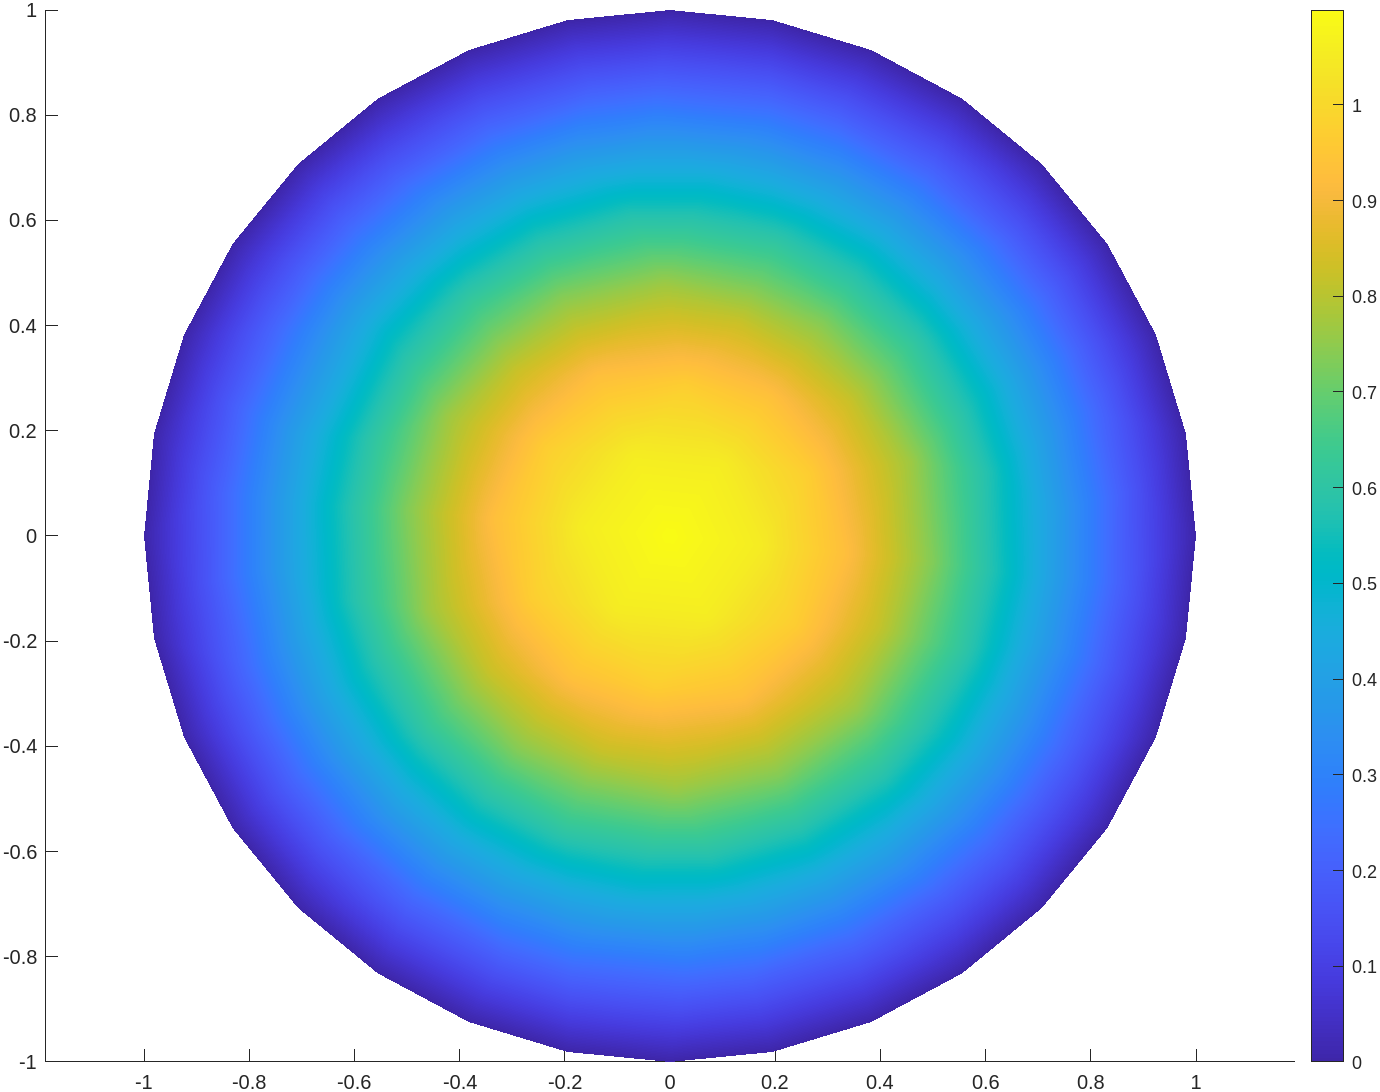
\includegraphics[width=0.4\textwidth]{lambda01}
  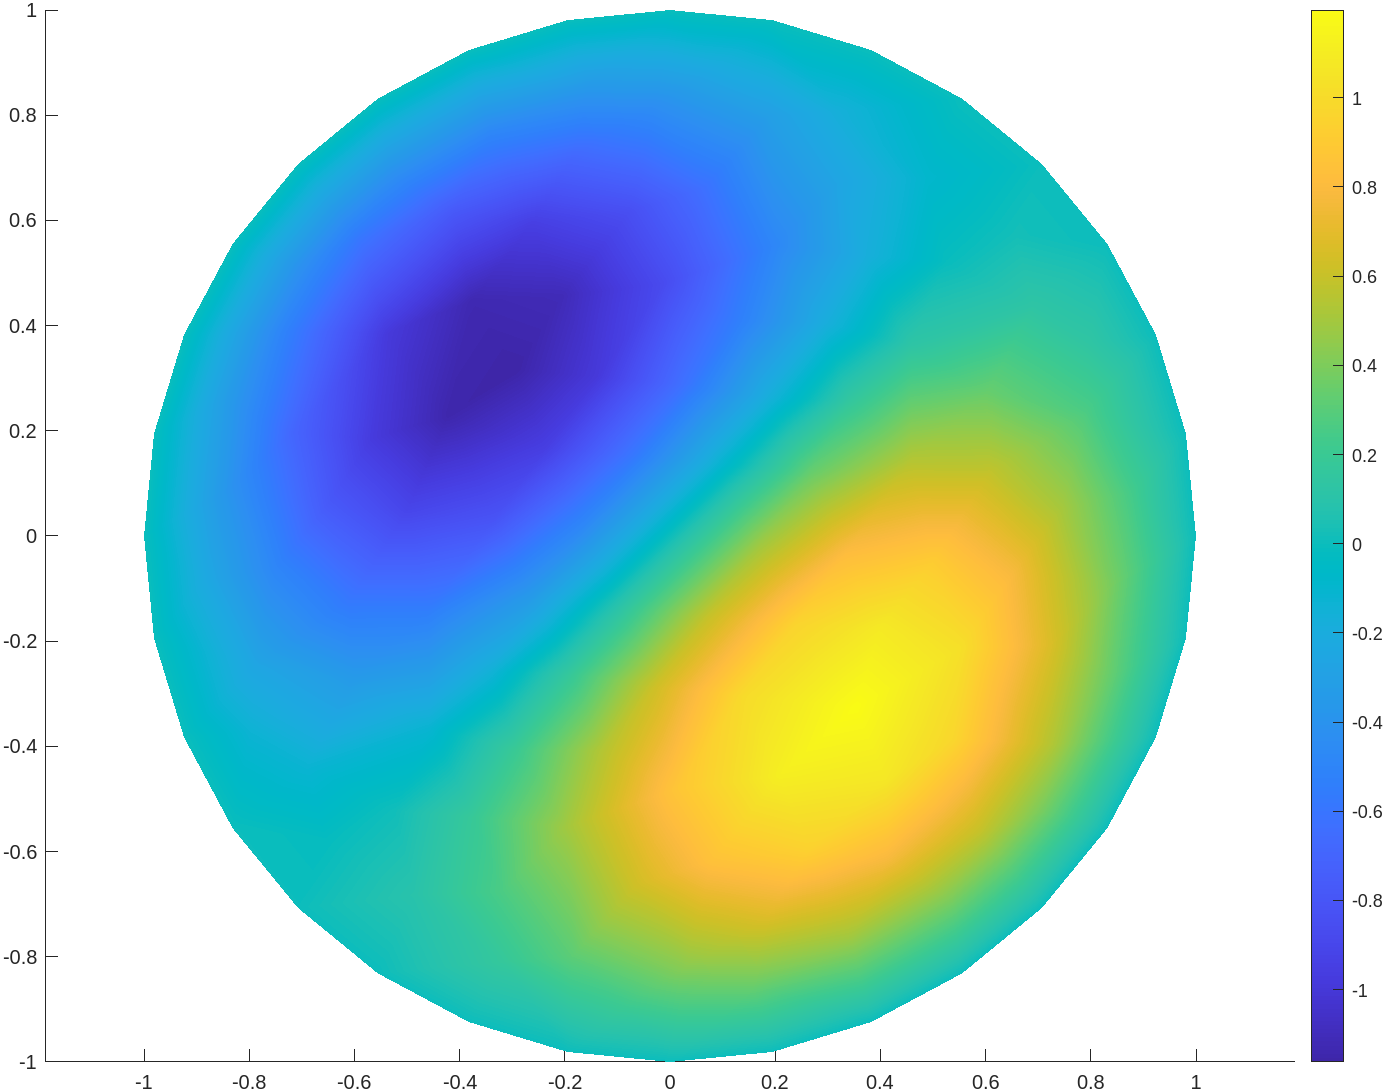
\includegraphics[width=0.4\textwidth]{lambda11}
  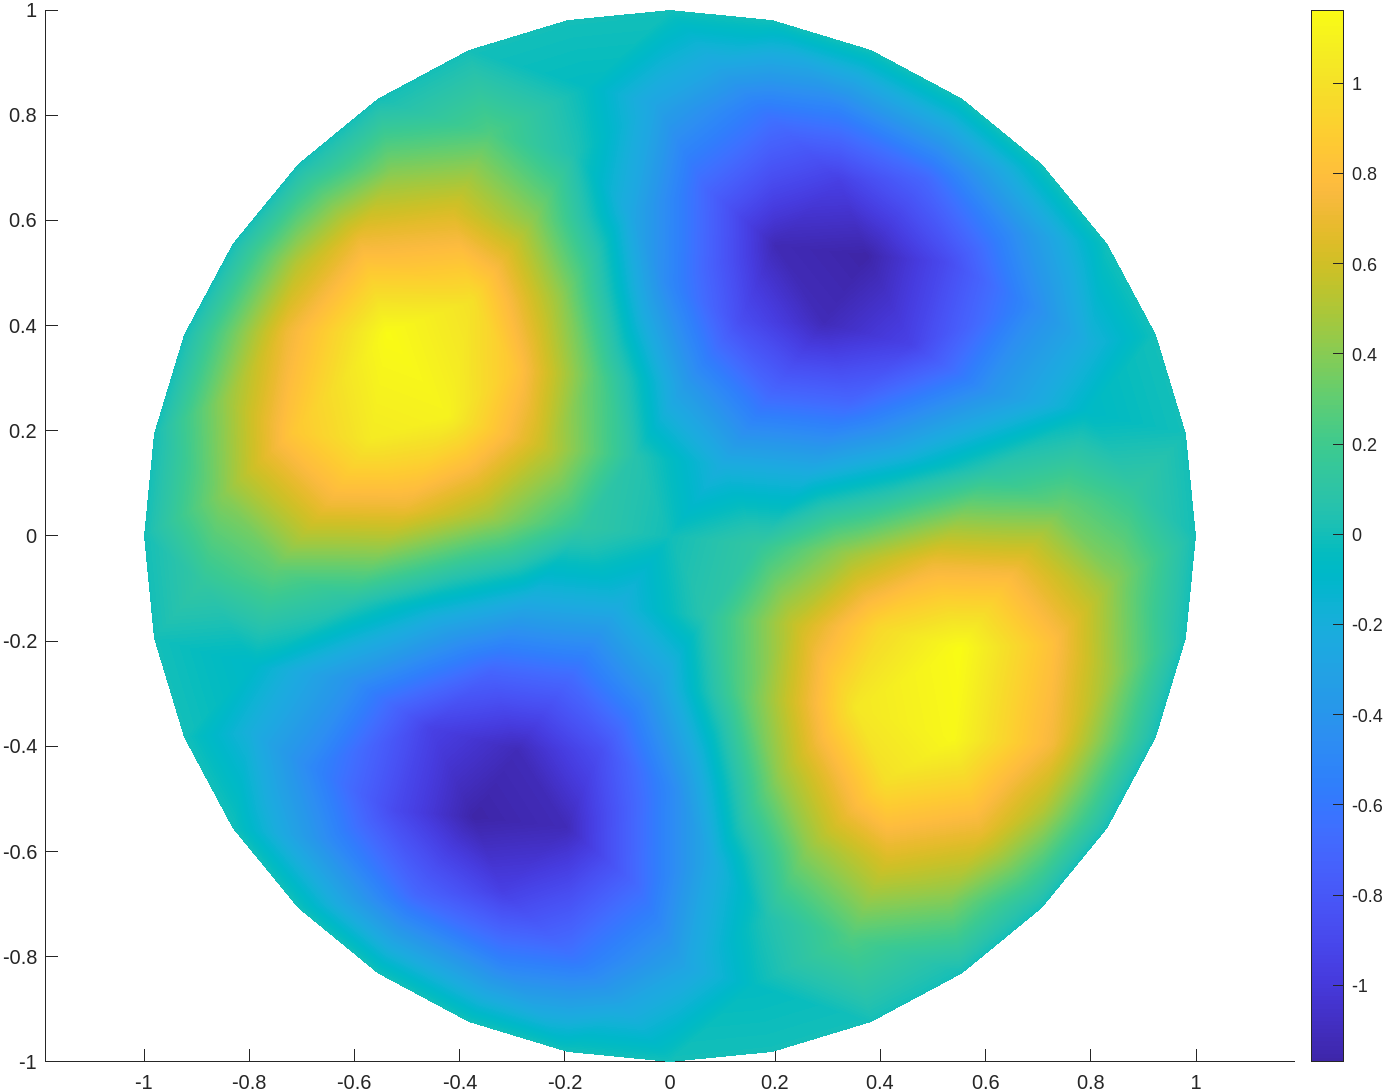
\includegraphics[width=0.4\textwidth]{lambda21}
  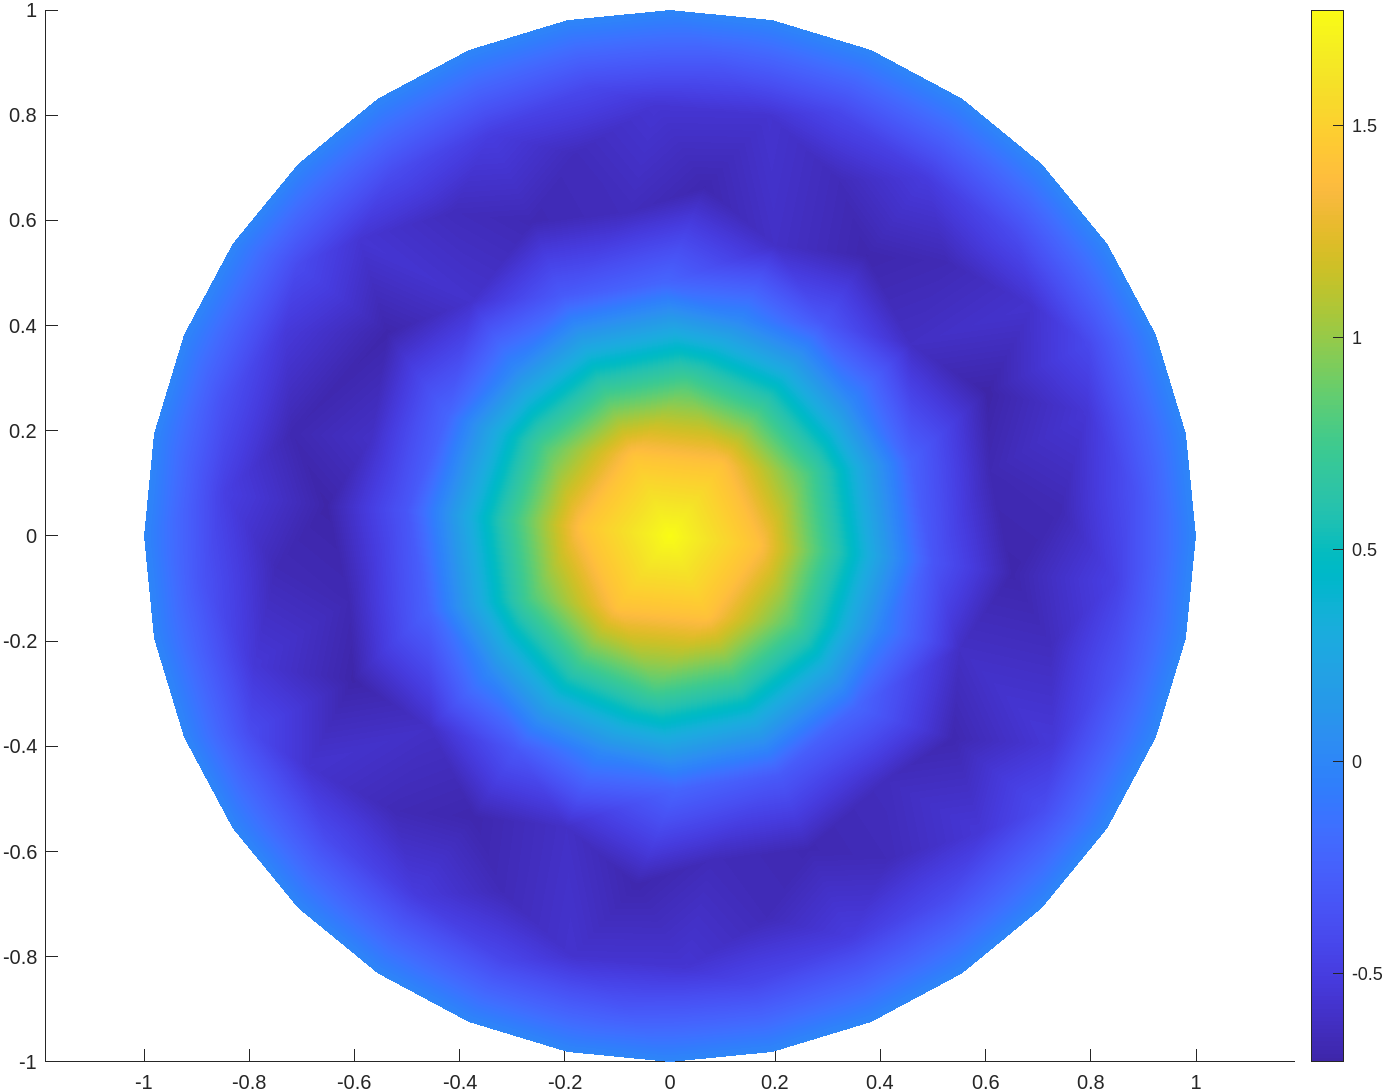
\includegraphics[width=0.4\textwidth]{lambda02}
  \caption{Plots for $\lambda_{0,1}$ (top left), $\lambda_{1,1}$ (top right)$,\lambda_{2,1}$ (bottom left) and $\lambda_{0,2}$ (bottom right).}
  \label{fig:q1}
\end{figure}

As for Richardson Extrapolation, we can use the following relationship:
\[
\lambda_N=\lambda_{\infty}+c_2\left(\frac{1}{N}\right)^2+O\left(\frac{1}{N^{4}}\right)
\]
\[
  \lambda_{2N}=\lambda_{\infty}+\frac{c_2}{4}\left(\frac{1}{N}\right)^2+O\left(\frac{1}{N^{4}}\right)
\]
\[
\implies\lambda_{\infty}=\frac{4\lambda_{2N}-\lambda_N}{3}+O\left( \frac{1}{N^{4}} \right) 
.\]

The code used for Richardson exptrapolation was as follows, and the results can be seen in table \ref{tab:q1}.
\begin{lstlisting}
eigrich = (4*eigenvalues64-eigenvalues32)/3;
\end{lstlisting}

\begin{table}[H]
\centering
\begin{tabular}{|c|c|c|c|}
\hline
Exact & FEM (32) & FEM (64) & Richardson Extrapolation \\ \hline
\(\lambda_{0,1} = 5.78318596\) & 5.858 & 5.8026 & 5.7843 \\ \hline
\(\lambda_{1,1} = 14.6819706\) & 15.126 & 14.8049 & 14.6946 \\ \hline
\(\lambda_{2,1} = 26.3746164\) & 27.879 & 26.7734 & 26.4050 \\ \hline
\(\lambda_{0,2} = 30.4712623\) & 32.538 & 31.0241 & 30.516 \\ \hline
\end{tabular}
\caption{Comparison of FEM results with the exact eigenvalues.}
\label{tab:q1}
\end{table}

\end{document}
